%Created with command:
%"/home/josh/Teaching/trunk/Utilities/makeexam" "Quiz 1" "Please show all work.  You may not use a calculator." "../NumberSystems/Assessments/convert_binary_decimal_qz.tex" "../NumberSystems/Assessments/convert_hex_oct_bin_qz.tex" "../NumberSystems/Assessments/twos_complement_arithmetic_qz.tex" "../CMOSCircuits/Assessments/cmos_buffer_design.tex"
\documentclass{article}
\usepackage[T1]{fontenc}
\usepackage{arev}
\usepackage{longtable}
\usepackage[hmargin=2cm,vmargin=2cm]{geometry}
\usepackage{graphicx}
\setlength{\parindent}{0pt}
\title{Quiz 1}
\date{}
\begin{document}
\maketitle
Please show all work.  You may not use a calculator. (16 points total)
\begin{longtable}[l]{rp{17cm}}
%file: ../NumberSystems/Assessments/convert_binary_decimal_qz.tex
1.&\begin{minipage}[t]{\linewidth}(2 pt) Convert the following binary numbers to decimal. \\
\\
$11110000_2$ \\
$01101100_2$ \\

Solution: \\
\\
$11110000_2 = 1 \cdot 2^7 + 1 \cdot 2^6 + 1 \cdot 2^5 + 1 \cdot 2^4 = 128 + 64 + 32 + 16 = 240$ \\
$01101100_2 = 1 \cdot 2^6 + 1 \cdot 2^5 + 1 \cdot 2^3 + 1 \cdot 2^2 = 64 + 32 + 8 + 4 = 108$ \\
\end{minipage}\\
\medskip
%file: ../NumberSystems/Assessments/convert_hex_oct_bin_qz.tex
2.&\begin{minipage}[t]{\linewidth}(4 pt) Perform the following number system conversions. \\
\\
$9\textrm{A}8\textrm{C} = ?_8$ \\
$10101011_2 = ?_{16}$ \\
$01010110_2 = ?_8$ \\
$737_8 = ?_2$ \\

Solution: \\
\\
$9\textrm{A}8\textrm{C} = 1001101010001100_2 = 001_2 001_2 101_2 010_2 001_2 100_2 = 115214_8$\\
$10101011_2 = 1010_2 1011_2 = \textrm{AB}_{16}$ \\
$01010110_2 = 001_2 010_2 110_2 = 126_8$ \\
$737_8 = 111_2 011_2 111_2 = 111011111_2$ \\
\\
\end{minipage}\\
\medskip
%file: ../NumberSystems/Assessments/twos_complement_arithmetic_qz.tex
3.&\begin{minipage}[t]{\linewidth}(6 pt) Perform the following binary arithmetic using the four bit two's complement representation, showing all carries.  For each case, determine if overflow occurs. If it does, state why it occurs.
\\
\\
$6 + -1$\\
$-4 - 5$\\

Solution: \\
\\
$6 = 0110_2$\\
$-1 = 1111_2$\\
\\
\begin{tabular}{cccccc}
  C & 1 & 1 & 1 & 0 & 0 \\
    &   & 0 & 1 & 1 & 0 \\
    & + & 1 & 1 & 1 & 1 \\
  \hline
    &   & 0 & 1 & 0 & 1 \\
\end{tabular} \\
\\
Overflow does not occur.\\
\\
$-4 = 1100_2$\\
$5 = 0101_2$\\
Note that $5$ complement is $1010_2$ and remember to use $c_{in}=1$.\\
\\
\begin{tabular}{cccccc}
  C & 1 & 0 & 0 & 0 & 1 \\
    &   & 1 & 1 & 0 & 0 \\
    & + & 1 & 0 & 1 & 0 \\
  \hline
    &   & 0 & 1 & 1 & 1 \\
\end{tabular} \\
\\
Overflow occurs because $c_{in} \neq c_{out}$ for MSB.\\
\end{minipage}\\
\medskip
%file: ../CMOSCircuits/Assessments/cmos_buffer_design.tex
4.&\begin{minipage}[t]{\linewidth}(4 pt) Write the function table and draw the circuit diagram for a one input CMOS noninverting buffer gate.  Note that this gate should use four transistors.\\ \\

Solution: \\ \\
\begin{tabular}{ccccccccc}
  \textbf{A} & \textbf{Q1} & \textbf{Q2} & \textbf{Q3} & \textbf{Q4} & \textbf{Z} \\
  \hline
  L & off & on & on & off & L\\
  H & on & off & off & on & H\\
\end{tabular} \\
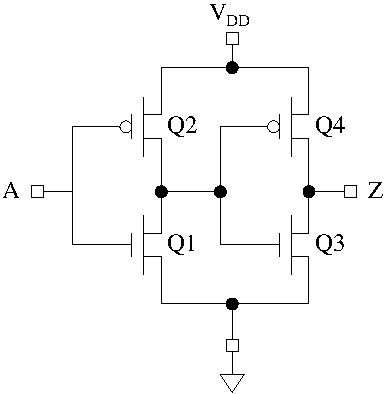
\includegraphics{../CMOSCircuits/Assessments/CMOSBufferGate}
\end{minipage}\\
\medskip
\end{longtable}
\end{document}
